%Arthur Tsuyoshi Sakano Vetori - 7990450
%        Victor Shin Kinoshita - 5947051

%pacotes

\documentclass[12pt]{article}

\usepackage[brazil]{babel} %hifenização em português do brasil
\usepackage[T1]{fontenc} % caracteres com acentos são considerados um bloco só
\usepackage{ae} %arruma a fonte quando usa o pacote acima
\usepackage[utf8x]{inputenc} % usa o utf8 para os caracteres
\usepackage{amssymb} %alguns caracteres matemáticos especiais
\usepackage[pdftex]{graphicx}%Para inserir figuras
\usepackage{breakurl} %usado para criar links de internet
\usepackage{url} %usado para criar links de internet
\usepackage{amssymb,amsmath}
\usepackage{MnSymbol}
\usepackage{mathdots}
%\usepackage{yhmath}

%documento
\begin{document}

\title{Laboratório de Computação e Simulação}
\author{Arthur Tsuyoshi Sakano Vetori - 7990450 \\ Victor Shin Kinoshita - 5947051}
\date{23/05/2013}
\maketitle

\begin{figure}[!h]
\begin{center}
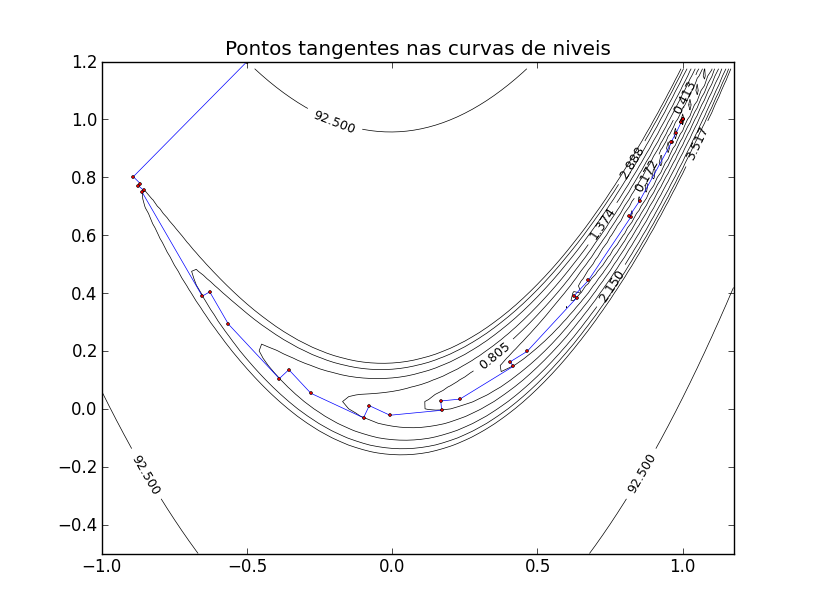
\includegraphics[width=14cm]{0_5_1_2_tangente.png}
\end{center}
\end{figure}

\newpage

%%%%%%%%%%%%%%%%%%%%%%%%%%%%%%%
%%%%%%%%% OBJETIVO %%%%%%%%%%%%
%%%%%%%%%%%%%%%%%%%%%%%%%%%%%%%

\section{Objetivo}
\mbox{}

Criar um algoritmo que encontra o mínimo de uma função com uma restrição $h(x) = 0$ usando busca linear por ajuste quadrático, ParTan e método da penalidade.


%%%%%%%%%%%%%%%%%%%%%%%%%%%%%%%
%%%%%%%%% DESENVOLVIMENTO %%%%%
%%%%%%%%%%%%%%%%%%%%%%%%%%%%%%%

\section{Desenvolvimento}
\mbox{}

Por padrão, usamos orientação a objetos para completarmos o objetivo. Usamos também o GitHub para versionar nosso programa e para ajudar no desenvolvimento em dupla. Para acessar o projeto completo, entre na página \url{https://github.com/vkinoshita/ep5.git}

Como estrutura do projeto, temos:

\begin{enumerate}
	\item ep5.py - programa principal. Ele que vai consumir todos os objetos para encontrar o mínimo da função.
	\item entrada.py - os valores de entrada que implementa a dimensão, a função, o gradiente, a restrição, o ponto inicial e o erro. 
	\item Pasta lib:
	\begin{enumerate}
		\item grg.py - possui o algoritmo que encontra o gradiente reduzido generalizado
		\item busca\_linear.py - responsável por encontrar o mínimo de uma função de acordo com uma direção dada. Ele implementa o ajuste quadrático como recurso pra encontrar o mínimo.
		\item partan.py - possui o algoritmo que encontra o mínimo da função.
		\item penalidade.py - implementa as funções do método da penalidade.
		\item saida.py - escreve o arquivo de saída.
	\end{enumerate}
	\item Pasta testes - possui todos os testes realizados durante o desenvolvimento do programa. Para executá-los, basta jogar todos os arquivos na mesma pasta que o ep5.py.
\end{enumerate}

Para realizarmos os testes, tomamos como referência os seguintes parâmetros com a seguinte função (Figura~\ref{funcao_teste}):

\begin{verbatim}
d = 3
m = 1
x0 = [1, 3, 10]
eps = 0.001

def f(x):
	fx = x[0]**2 + 2*(x[1]**2) + 3*(x[2]**2)
	return(fx)

def g(x):
	gx = [2*x[0], 4*x[1], 6*x[2]]
	return(gx)

def h(x):
	hx = [x[0]**2 +x[1] -5*x[2]]
	return(hx)

def j(x):
	jx = [[2*x[0], 1, -5]]
	return(jx)
\end{verbatim}

\begin{figure}[!h]
\centering
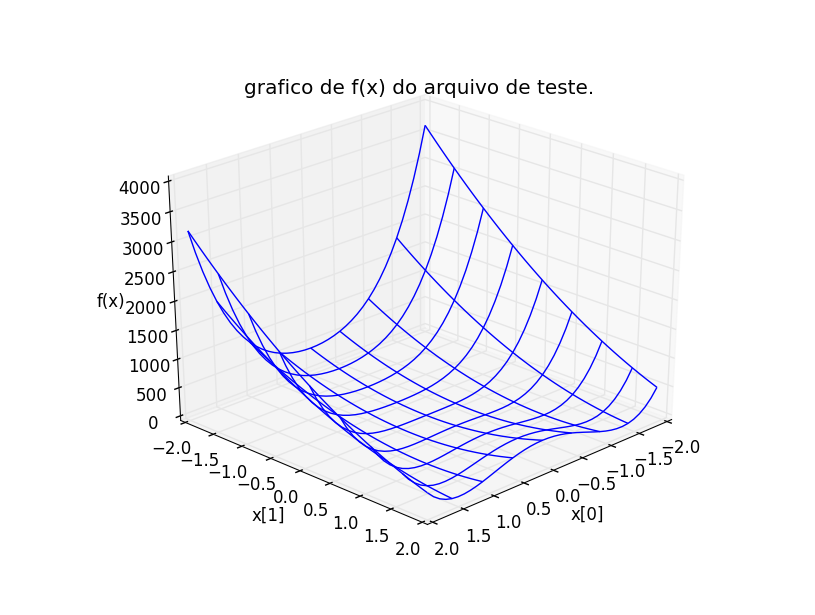
\includegraphics[width=14cm]{funcao_teste.png}
\caption{Função usada para o teste}
\label{funcao_teste}
\end{figure}



%%%%%%%%%%%%%%%%%%%%%%%%%%%%%%%
%%% SOBRE O ALGORITMO %%%%%%%%%
%%%%%%%%%%%%%%%%%%%%%%%%%%%%%%%

\section{Sobre o Algoritmo}
\mbox{}

O programa basicamente realiza as seguintes etapas:

\begin{enumerate}
	\item Leitura do arquivo de entrada.
	\item Busca do valor mínimo pelo ParTan usando a busca linear por ajuste quadrático.
	\item Escrita do arquivo de saída
\end{enumerate}

%%%%%%%%%%%%%%%%%%%%%%%%%%%%%%%
%%%%%%%% BUSCA LINEAR %%%%%%%%%
%%%%%%%%%%%%%%%%%%%%%%%%%%%%%%%

\section{Busca Linear}
\mbox{}

A busca linear consiste na influência de um elemento sobre o próximo. Para a etapa $k$, uma posição $x_{k}$ e uma certa direção $d$, resumidamente temos que

\begin{equation} \label{eq:posicao_x}
x_{k + 1} = x_{k} + \eta_{k}d
\end{equation}

Assim, temos uma função para cada posição de $\eta$

\begin{equation} \label{eq:equacao_phi}
g(\eta) = f(x_{k} + \eta d)
\end{equation}

Entre os diversos tipos de busca linear, o que muda, é a forma em que o $x_{k + 1}$ é encontrado.

\subsection{Ajuste Quadrático}
\mbox{}

O ajuste quadrático consiste em interpolar 3 pontos previamente escolhidos para uma função quadrática. Durante as etapas, o algoritmo realiza perturbações nesses 3 pontos, sempre tentando encontrar o menor valor.

Em outras palavras, inicialmente são ``chutados" os pontos $\{\eta_1, \eta_2, \eta_3\}$, com seus respectivos valores

\[ \left\{ 
\begin{array}{l} 
	\phi_1 = g(\eta_1) = f(x_0 + \eta_1 d) \\
	\phi_2 = g(\eta_2) = f(x_0 + \eta_2 d) \\
	\phi_3 = g(\eta_3) = f(x_0 + \eta_3 d) \\
\end{array} \right.\] \\

Satisfazendo as seguintes condições

\begin{equation} \label{eq:condicao_eta}
	\eta_1 < \eta_2 < \eta_3 
\end{equation} 
\begin{equation} \label{eq:condicao_phi}
	\phi_1 \geq \phi_2 \leq \phi_3
\end{equation} \\

os pontos ficam prontos para serem usados na interpolação da função quadrática.

\subsection{Interpolação}
\mbox{}

A função será dada por

\begin{equation}
	\phi(\eta) = a\eta^2 + b\eta + c
\end{equation} \\

Como já temos $\{\eta_1, \eta_2,\eta_3\}$ e $\{\phi_1, \phi_2, \phi_3\}$, manipulando algebricamente, encontramos que

\begin{equation}
a = \frac{(\eta_2 - \eta_3)\phi_1 + (\eta_3 - \eta_1)\phi_2 + (\eta_1 - \eta_2)\phi_1}{-(\eta_2 - \eta_1)(\eta_3 - \eta_2)(\eta_3 - \eta_1)} 
\end{equation}

\begin{equation}
b = \frac{(\eta_3^2 - \eta_2^2)\phi_1 + (\eta_1^2 - \eta_3^2)\phi_2 + (\eta_2^2 - \eta_1^2)\phi_1}{-(\eta_2 - \eta_1)(\eta_3 - \eta_2)(\eta_3 - \eta_1)} 
\end{equation}

\begin{equation}
c = \frac{(\eta_3\eta_2^2 - \eta_2\eta_3^2)\phi_1 + (\eta_1\eta_3^2 - \eta_3\eta_1^2)\phi_2 + (\eta_2\eta_1^2 - \eta_1\eta_2^2)\phi_1}{- (\eta_2 - \eta_1)(\eta_3 - \eta_2)(\eta_3 - \eta_1)} 
\end{equation} \\

Agora, basta encontrar o $\eta$ mínimo, tal que $g'(\eta) = 0$. Como é uma função de segundo grau, facilmente, temos que o ponto mais baixo é dado por

\begin{equation} \label{eq:eta_minimo}
\eta_{min} = -\frac{b} {2 a}
\end{equation} \\

\subsection{Trinca inicial}
\mbox{}

Para que a busca funcione, é fundamental encontrar os $\eta s$ iniciais. Fizemos então, uma trinca inicial $\{-0.0005, 0, 0.0005\}$ e moldamos ele ao ponto de satisfazer $\eta_1 < \eta_2 < \eta_3$ e $\phi_1 \geq \phi_2 \leq \phi_3$.

Foi feito, para um $\alpha > 1$:

\begin{enumerate}
	\item Enquanto $\phi_1 < \phi_2$, $\eta_1$ recebe $\eta_1\alpha$.
	\item Enquanto $\phi_3 < \phi_2$, $\eta_3$ recebe $\eta_3\alpha$.
\end{enumerate}

Assim, multiplicamos cada uma das pontas por uma constante até que os pontos fiquem bons.

\subsection{Perturbações}
\mbox{}

As perturbações são sempre baseadas no valor encontrado por \eqref{eq:eta_minimo}.

Como a meta do algoritmo é encontrar o mínimo de uma função, à partir do momento que temos $\eta_{min}$ e $\phi_{min} = g(\eta_{min})$, geramos novas trincas $\{\eta_1, \eta_2, \eta_3\}$ e $\{\phi_1, \phi_2, \phi_3\}$, sempre satisfazendo as condições \eqref{eq:condicao_eta} e \eqref{eq:condicao_phi}. Ou seja,

\begin{enumerate}
	\item Se $\eta_{min} > \eta_2$:
	\begin{enumerate}
		\item Se $\phi_{min} > \phi_2$, escolhemos as trincas novas $\{\eta_1, \eta_2, \eta_{min}\}$ e $\{\phi_1, \phi_2, \phi_{min}\}$.
		\item caso contrário, escolhemos as trincas novas $\{\eta_2, \eta_{min}, \eta_3\}$ e $\{\phi_2, \phi_{min}, \phi_3\}$.
	\end{enumerate}
	\item Se $\eta_{min} \leq \eta_2$:
	\begin{enumerate}
		\item Se $\phi_{min} > \phi_2$, escolhemos as trincas novas $\{\eta_{min}, \eta_2, \eta_3\}$ e $\{\phi_{min}, \phi_2, \phi_3\}$.
		\item caso contrário, escolhemos as trincas novas $\{\eta_1, \eta_{min}, \eta_2\}$ e $\{\phi_1, \phi_{min}, \phi_2\}$.
	\end{enumerate}
\end{enumerate}

Observe que as trocas sempre priorizam as condições \eqref{eq:condicao_eta} e \eqref{eq:condicao_phi} e, ao mesmo tempo, adicionam um ponto menor sem denegrir a função original $g(\eta)$. Ou seja, ele sempre vai em direção ao ponto de menor valor.

\subsection{Erro}
\mbox{}

Para garantir a qualidade do resultado, foi estipulado a seguinte condição de erro:

\begin{equation}
	|\eta_{min} − \eta_2| < \epsilon
\end{equation}

Ou seja, se as perturbações começarem a gerar pontos pouco distantes (menores que $\epsilon$), garantimos então que $\eta$ não irá variar mais que $\epsilon$.

No programa, como foi observado comportamentos muito indesejáveis em pontos distantes, foi adotado um $\epsilon = 0.0000001$ para que ele consiga resultados consistentes no partan. Não foi usado o $\epsilon$ de entrada do programa (entrada.py) com o propósito de que o algoritmo aceite o máximo de pontos possíveis, reservando esse erro apenas para o ParTan, que será descrito na próxima seção.

\subsection{Algoritmo da Busca Linear por Ajuste Quadrático}
\mbox{}

Juntando todos os conceitos anteriores, temos o algoritmo:

\begin{enumerate}
	\item Encontrar as trincas iniciais $\{\eta_1, \eta_2,\eta_3\}$ e $\{\phi_1, \phi_2, \phi_3\}$.
	\item Gerar $\eta_{min}$ e $\phi_{min}$ à partir da trinca inicial.
	\item Se $|\eta_{min} − \eta_2| < \epsilon$, retornar $\eta_{min}$, caso contrário:
	\begin{enumerate}
		\item Atualizar a trinca com $\eta_{min}$ e $\phi_{min}$. (Dado na seção ``Perturbações").
		\item Gerar $\eta_{min}$ e $\phi_{min}$ à partir da trinca atual.
		\item Voltar para o item 3.
	\end{enumerate}
\end{enumerate}

\subsection{Resultados}
\mbox{}

Como esperado, o algoritmo encontra o mínimo de forma consistente. Sendo que, quanto mais o ponto está longe do mínimo, mais ele demora pra chegar. Como no caso do [2, -2] que precisou de menos de 10 iterações pra convergir e no caso do [100, 100] que precisou de muito mais pontos para estabilizar. 

\clearpage
\subsubsection{Início em [2, -2] para 10 iterações}
\mbox{}

\begin{figure}[!h]
\begin{center}
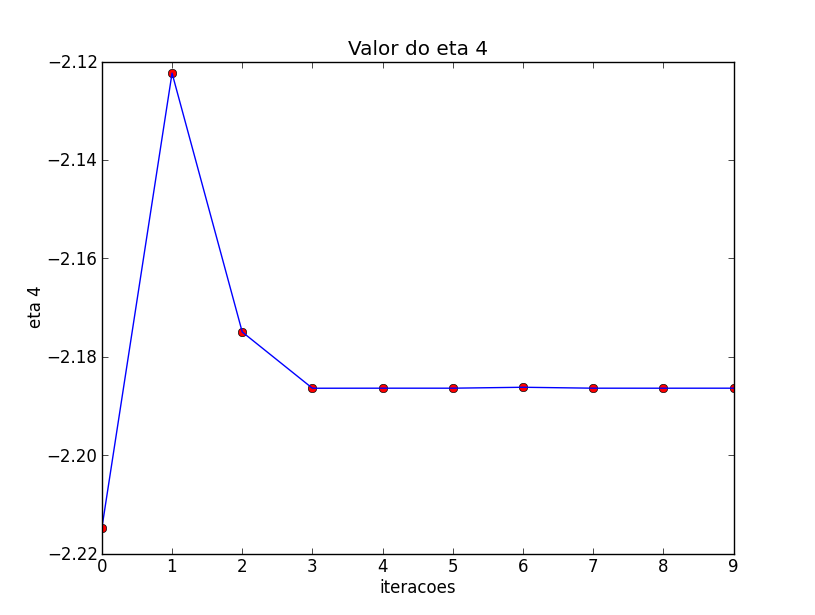
\includegraphics[width=10cm]{2_2_eta_4.png}
\end{center}
\end{figure}

\begin{figure}[!h]
\begin{center}
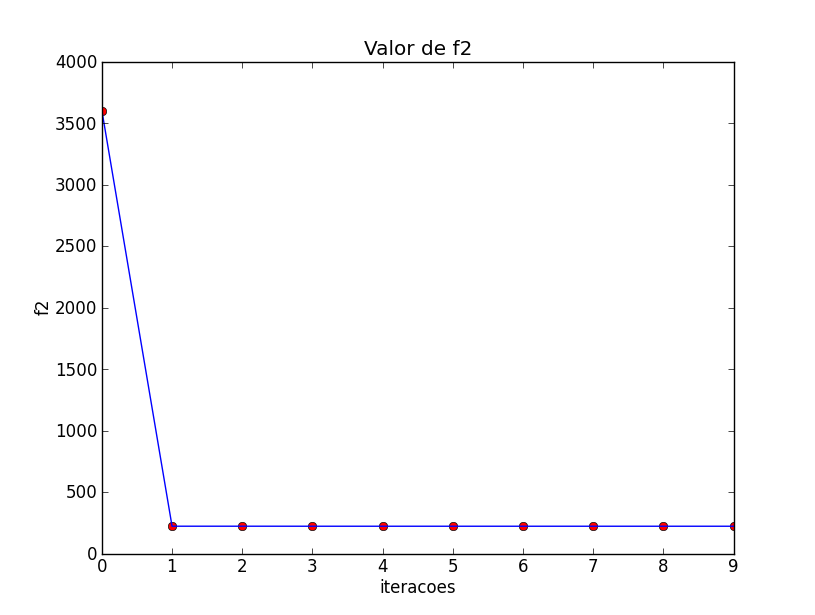
\includegraphics[width=10cm]{2_2_f_2.png}
\end{center}
\end{figure}

\begin{figure}[!h]
\begin{center}
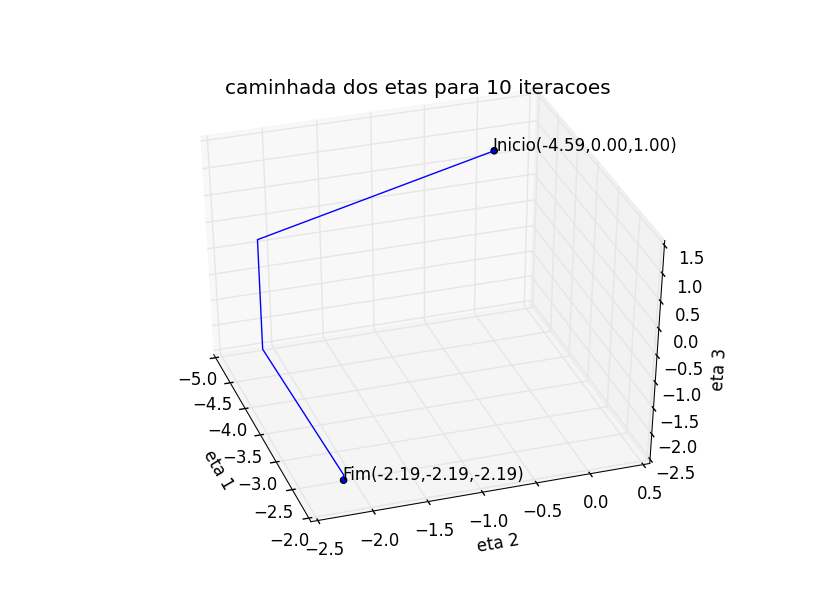
\includegraphics[width=12cm]{2_2_caminhada.png}
\end{center}
\end{figure}

\clearpage
\subsubsection{Início em [0, 0] para 50 iterações}
\mbox{}

\begin{figure}[!h]
\begin{center}
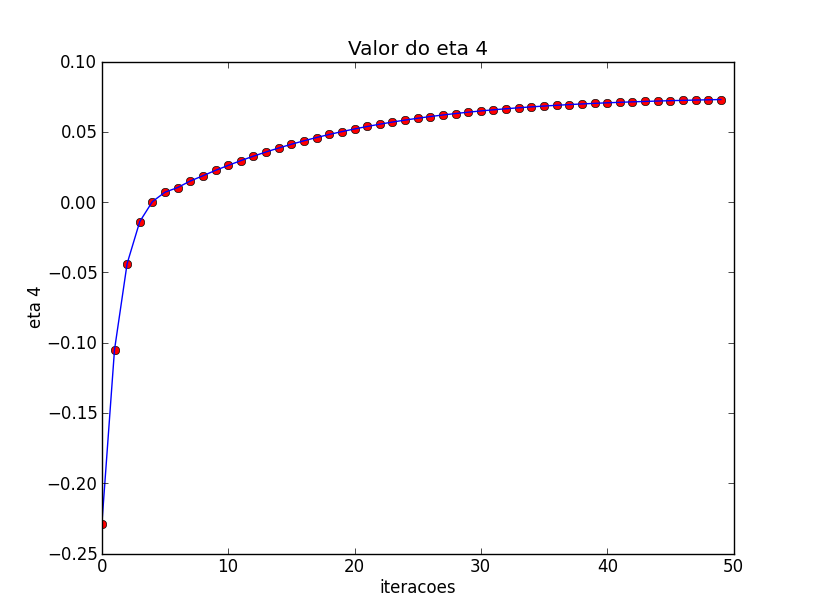
\includegraphics[width=10cm]{0_0_eta_4.png}
\end{center}
\end{figure}

\begin{figure}[!h]
\begin{center}
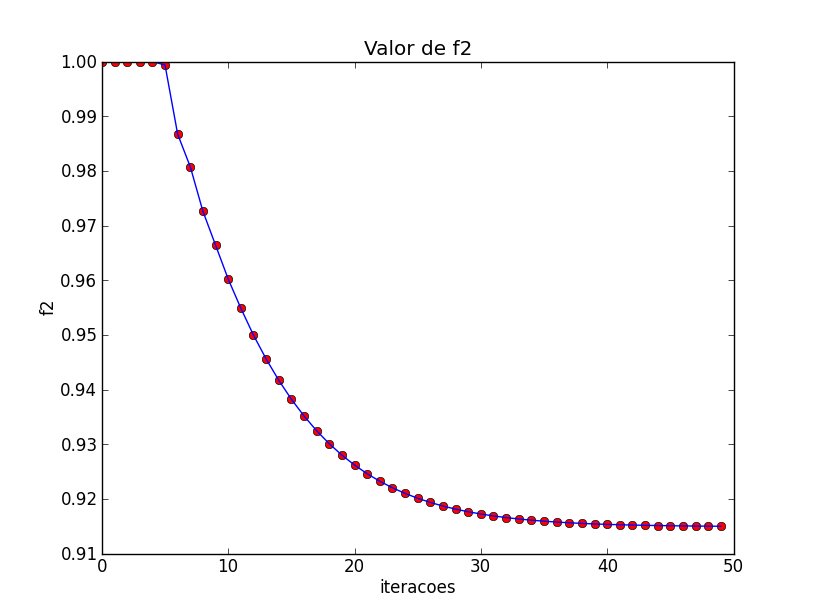
\includegraphics[width=10cm]{0_0_f_2.png}
\end{center}
\end{figure}

\begin{figure}[!h]
\begin{center}
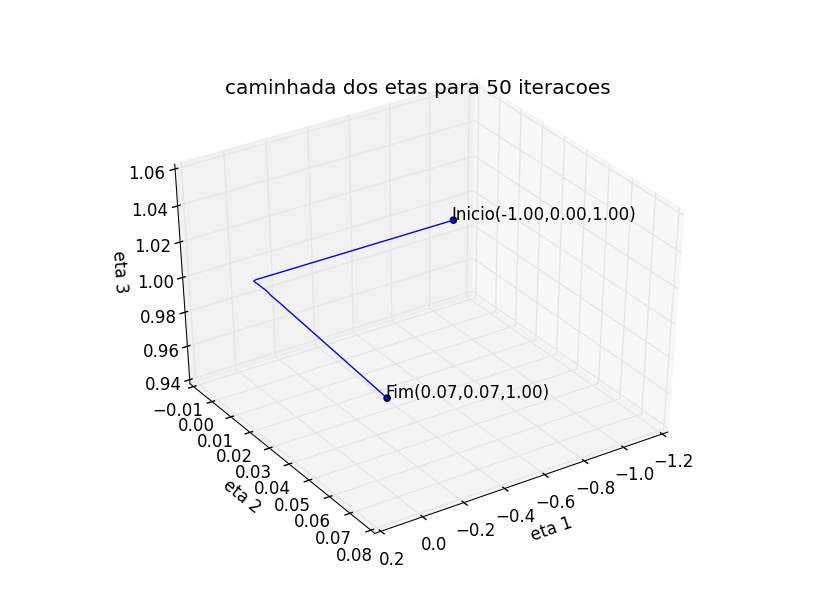
\includegraphics[width=12cm]{0_0_caminhada.png}
\end{center}
\end{figure}

\clearpage
\subsubsection{Início em [20, 20] para 100 iterações}
\mbox{}

\begin{figure}[!h]
\begin{center}
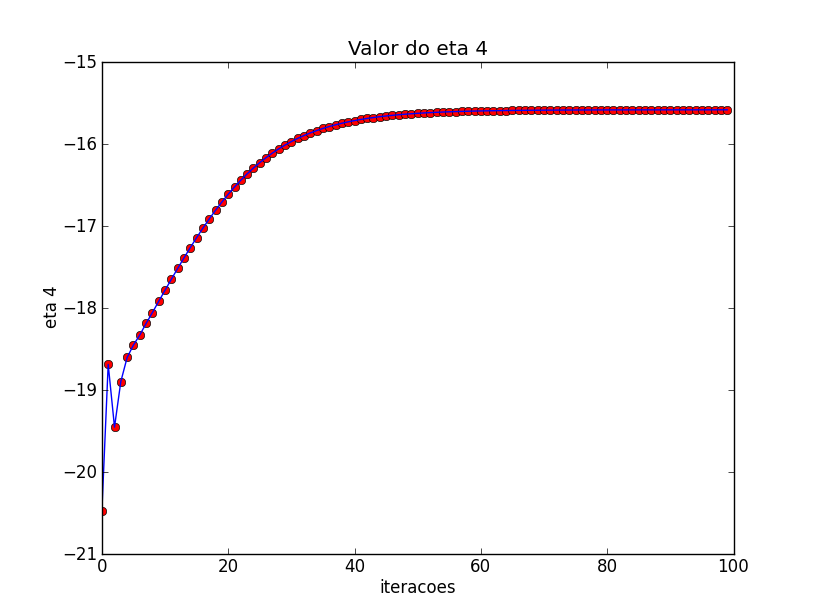
\includegraphics[width=10cm]{20_20_eta_4.png}
\end{center}
\end{figure}

\begin{figure}[!h]
\begin{center}
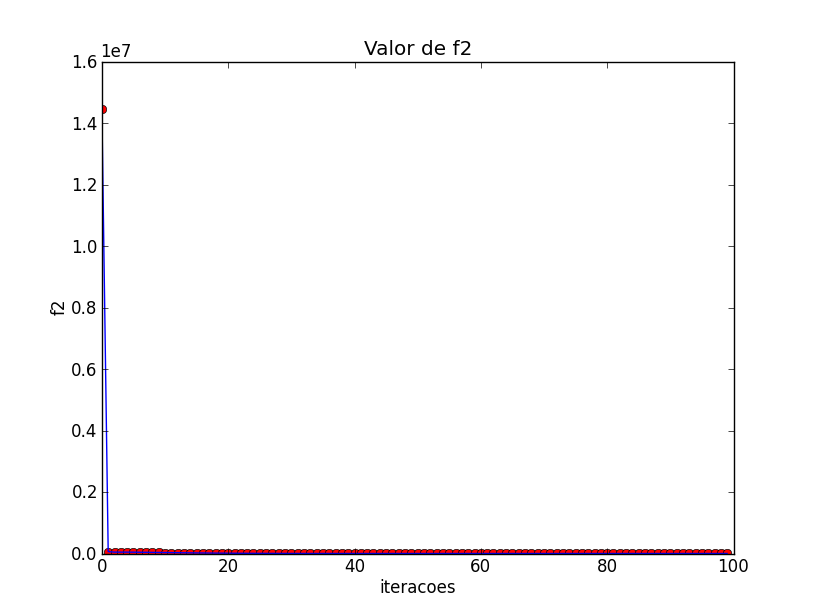
\includegraphics[width=10cm]{20_20_f_2.png}
\end{center}
\end{figure}

\begin{figure}[!h]
\begin{center}
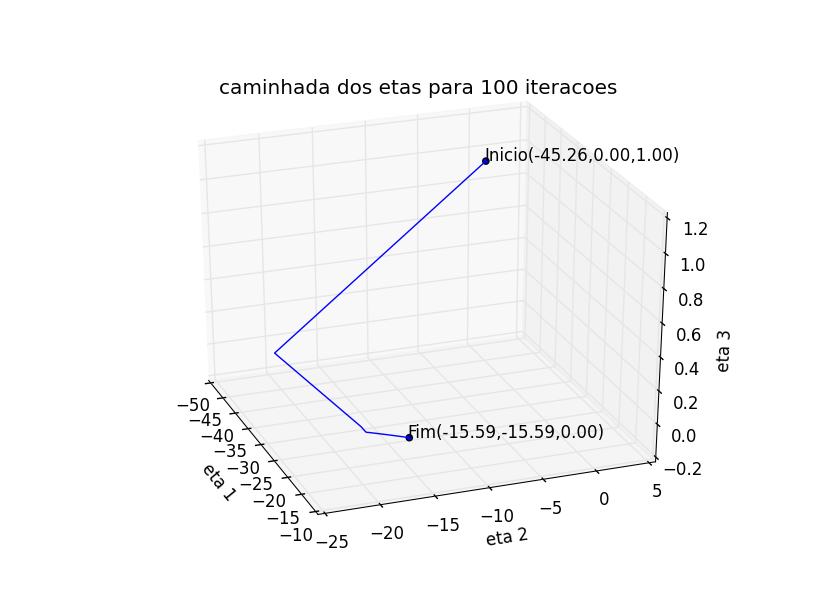
\includegraphics[width=12cm]{20_20_caminhada.png}
\end{center}
\end{figure}

\clearpage
\subsubsection{Início em [100, 100] para 500 iterações}
\mbox{}

\begin{figure}[!h]
\begin{center}
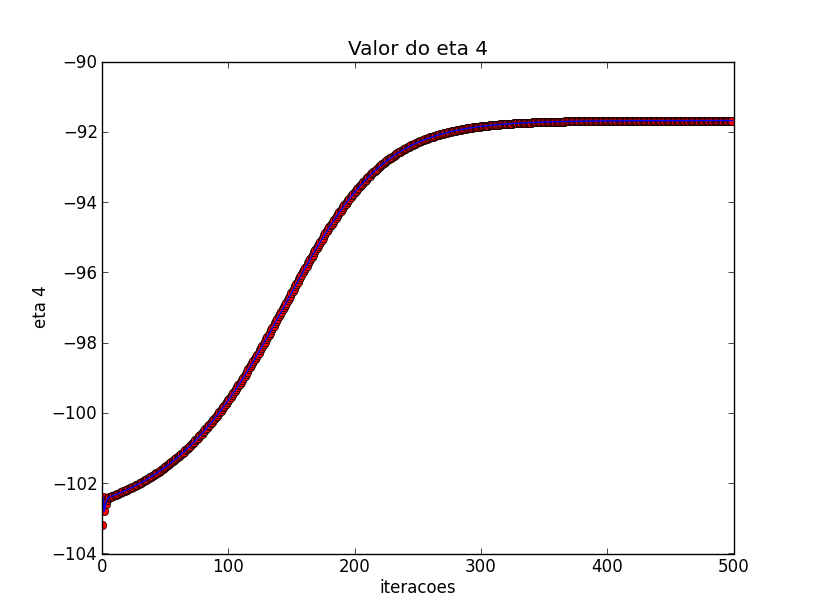
\includegraphics[width=10cm]{100_100_eta_4.png}
\end{center}
\end{figure}

\begin{figure}[!h]
\begin{center}
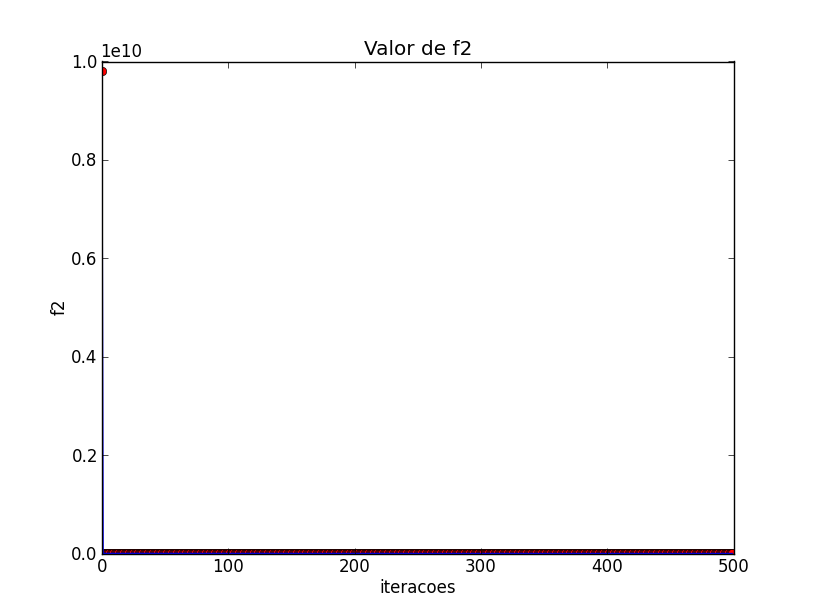
\includegraphics[width=10cm]{100_100_f_2.png}
\end{center}
\end{figure}

\begin{figure}[!h]
\begin{center}
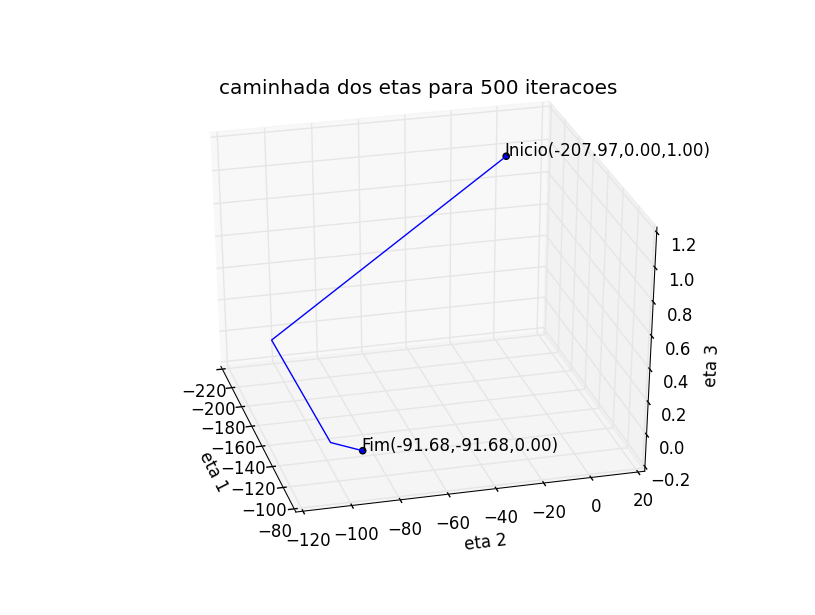
\includegraphics[width=12cm]{100_100_caminhada.png}
\end{center}
\end{figure}

%%%%%%%%%%%%%%%%%%%%%%%%%%%%%%%
%%%%%%%%%% PARTAN %%%%%%%%%%%%%
%%%%%%%%%%%%%%%%%%%%%%%%%%%%%%%

\clearpage
\section{ParTan}
\mbox{}

\subsection{Minimização em $R^{2}$}
\mbox{}

O método das Tangentes Paralelas(ParTan) foi utilizado para a minimização de uma função $f : R^{2} \rightarrow R$. O método consiste em, a cada iteração, a partir de um ponto $x_{0}$ dado, passar uma reta pelo ponto inicial e pelo ponto que minimiza a função ao longo da direção.

\subsection{ParTan - descrição}
\mbox{}

Considerando um problema em minimizar uma função $f(x)$ sobre todo $x \epsilon E^{n}$ onde $E^{n}$ é o espaço Euclidiano n-dimensional real. O procedimento ParTan pode ser descrito recursivamente da seguinte forma:

$k = 0:$

$$x^{1} = x^{0} - \mu^{0}\nabla f(x^{0})$$ 

onde $\mu^{0} = argmin \lbrace f(x^{0} - \mu\nabla f(x^{0}))\rbrace$ \\

Para $k \geqslant 1:$

$$v^{k} = x^{k} - \mu^{k}\nabla f(x^{k})$$

onde $\mu^{k} = argmin\lbrace f(x^{k} - \mu\nabla f(x^{k}))\rbrace$

$$x^{k+1} =  x^{k+1} + \omega^{k}[v^{k} - x^{k-1}]$$

onde $\omega^{k} = argmin\lbrace f(x^{k-1} + \omega(v^{k} - x^{k-1}))\rbrace$\\

Desde que $x^{1} - x^{0}$ esteja sobre o gradiente negativo, $x^{1} - x^{0}$ é perpendicular à tangente em $x^{0}$. Desde que $x^{1}$ é o ponto mínimo sobre  $x^{1} - x^{0}$ e $v^{1} - x^{1}$ esteja sobre o gradiente negativo, então $v^{1} - x^{1}$ é perpendicular a  $x^{1} - x^{0}$. Consequentemente, $v^{1} - x^{1}$ é paralela à tangente no ponto $x^{0}$. Desde que $v^{1}$ seja o mínimo sobre $v^{1} - x^{1}$, a tangente em $v^{1}$ contêm a reta $v^{1} - x^{1}$, na qual implica que a tangente no ponto $x^{0}$ é paralela à tangente em $v^{1}$. Portanto, $x^{2}$ é o ponto de mínimo sobre a direção $v^{1} - x^{0}$, e também, o ponto de mínimo da função quadrática. 

\subsection{Condição de Parada}
\mbox{}

A condição de parada utilizada foi:

$$ ||\nabla f(x^{0})|| < \epsilon $$ onde $\epsilon$ é o erro desejado definido inicialmente pela entrada do programa.\\

Ou seja, quando a norma do gradiente de $x^{0}$ for menor que o erro, significa que o ponto desejado foi encontrado.

\subsection{Algoritmo de ParTan}
\mbox{}
Procedimento:

\begin{enumerate}
	\item Definir um ponto $x_{0}$ inicial e fazer $x = x_{0}$
	\item Enquanto $||\nabla f(x)|| > \epsilon$, onde $\epsilon$ é o erro, repetir:
	\begin{enumerate}
		\item Busca linear no ponto $x$ na direção $\nabla f(x)$, encontrando o ponto $p_0$.
		\item Busca linear no ponto $p_0$ na direção $\nabla f(p_0)$, encontrando o ponto $p_1$.
		\item Fazer $d = p_1 - x$ depois busca linear no ponto $x$ na direção $\nabla f(d)$, encontrando um novo ponto para $x$
	\end{enumerate}
\end{enumerate}

\subsection{Representação gráfica do comportamento do ParTan}
\mbox{}

Realizando testes com a função de exemplo, ficou evidente que os pontos tangenciam cada curva de nível, sempre encontrando o menor ponto possível.

\clearpage
\subsubsection{Início em [-0.5, 1.2]}

\begin{figure}[!h]
\begin{center}
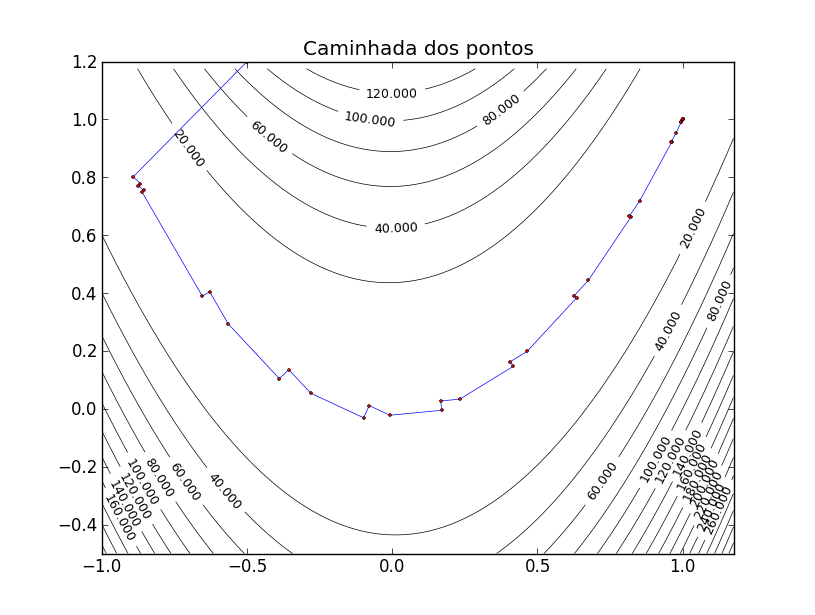
\includegraphics[width=10cm]{0_5_1_2_partan.png}
\end{center}
\end{figure}

\begin{figure}[!h]
\begin{center}
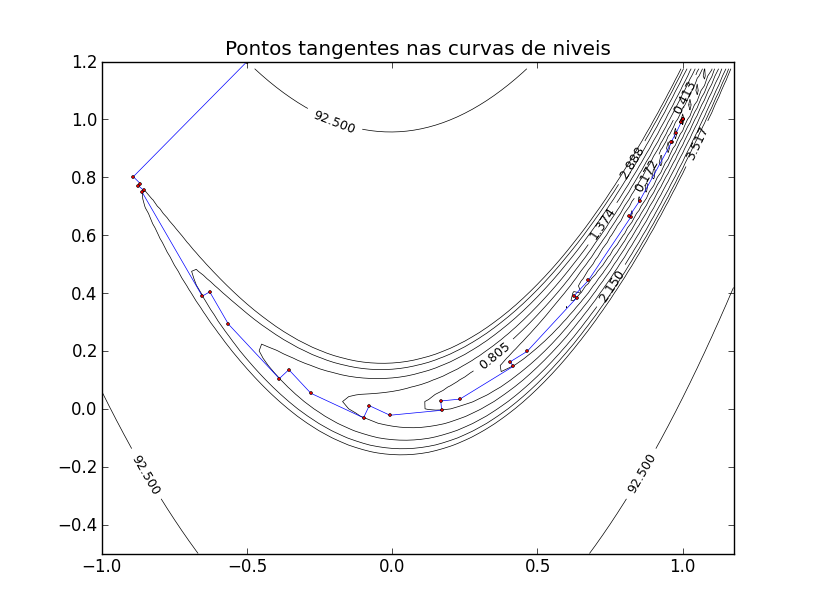
\includegraphics[width=10cm]{0_5_1_2_tangente.png}
\end{center}
\end{figure}

\clearpage
\subsubsection{Início em [2, -2]}

\begin{figure}[!h]
\begin{center}
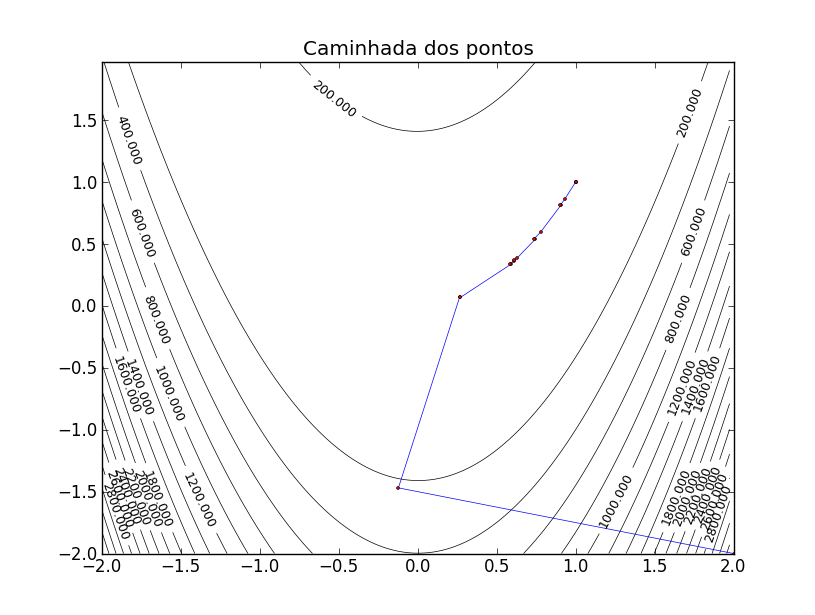
\includegraphics[width=10cm]{2_2_partan.png}
\end{center}
\end{figure}

\begin{figure}[!h]
\begin{center}
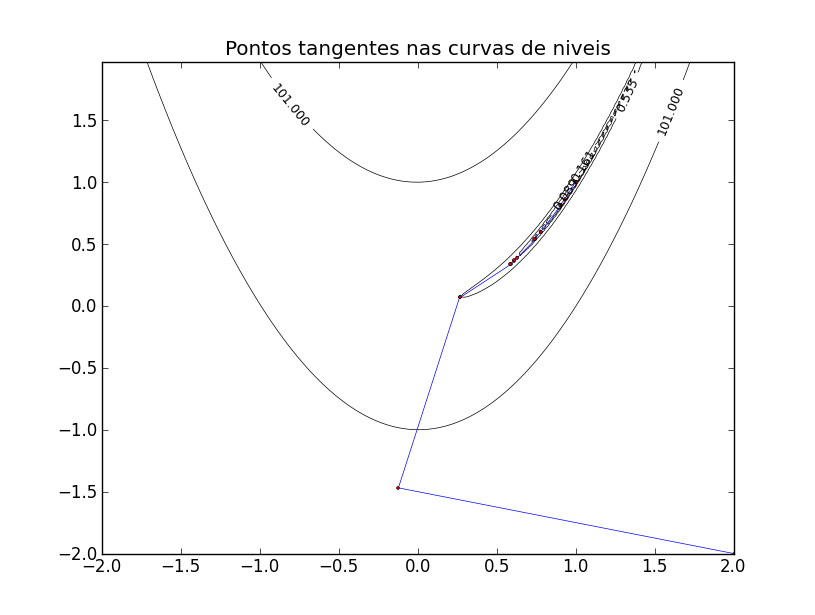
\includegraphics[width=10cm]{2_2_tangente.png}
\end{center}
\end{figure}

\newpage


%%%%%%%%%%%%%%%%%%%%%%%%%%%%%%%
%%%%%%%%% RESULTADOS %%%%%%%%%%
%%%%%%%%%%%%%%%%%%%%%%%%%%%%%%%

\section{Resultados do ParTan}
\mbox{}

Juntando o ParTan e a Busca Linear, tivemos resultados satisfatórios.

\begin{verbatim}
entrada.py

x = [2, -2]
argumento otimo = [1.0001283267248189, 1.000256585231958]
valor otimo = 1.64684654649e-08


x = [20, -3]
argumento otimo = [0.99999901590570672, 0.99999808130539891]
valor otimo = 1.21339745142e-12

x = [1, 1] # é o próprio mínimo
argumento otimo = [1, 1]
valor otimo = 0

x = [100, 100]
argumento otimo = [1.00000039736144, 1.0000008221948953]
valor otimo = 2.33366409184e-13

x = [-100, 100]
argumento otimo = [0.99999997463153278, 0.99999993370986051]
valor otimo = 2.48337799561e-14

x = [-200, 200]
argumento otimo = [0.99996538160948201, 0.99993193640225708]
valor otimo = 1.3357878133e-09

x = [-200, 300]
argumento otimo = [0.99999997979362665, 0.9999999599657462]
valor otimo = 4.2262317825e-16


#testes feitos com diferentes funções e diferentes dimensões
#entrada.py e entrada5.py são de dimensão 2
#entrada2.py e entrada3.py são de dimensao 3
#entrada4.py é de dimensão 4
#os arquivos estão na pasta teste

entrada.py
x = [2, -2]
argumento otimo = [1.0001283267248189, 1.000256585231958]
valor otimo = 1.64684654649e-08

entrada2.py 
x = [3, -2, -10]
argumento otimo = [-4.2515391632884002e-05, -0.00025509234979765683, 
    -1.8895729615115498e-06]
valor otimo = 1.80836188505e-08

entrada3.py
x = [20, -2, 7.43]
argumento otimo = [1.0000498288148181, 1.000099899787638, 
    1.3994559549746369e-05]
valor otimo = 2.53761712535e-09

entrada4.py
x = [-2, 2, 2, 2]
argumento otimo = [0.99907342705390434, 0.99814390466666225, 
    2.7409407719371738e-05, -0.0001747125669226792]
valor otimo = 9.28855395766e-07

entrada5.py
x = [10, -10]
argumento otimo = [3.5527136788005009e-15, 1.7763568394002505e-14]
valor otimo = 50.0

\end{verbatim}

%%%%%%%%%%%%%%%%%%%%%%%%%%%%%%%
%%%%%%%%%%%%% GRG %%%%%%%%%%%%%
%%%%%%%%%%%%%%%%%%%%%%%%%%%%%%%

\section{Método da Penalidade}
\mbox{}

Considere o seguinte problema:
$$Minimizar \, f(x)$$
$$Sujeita \, a\, h(x) = 0$$

Onde $f:R^{n} \rightarrow R$ e $h:R^{n} \rightarrow R^{l}$ são diferenciáveis.
Seja $\mu > 0$ um parâmetro de penalidade, ou seja, um peso dado para a restrição, e considere o problema de penalidade para minimizar $q(x)$ sujeita a $x\, \epsilon \, R^{n}$, onde $q(x) = f(x) + \mu \sum^{l}_{i=1} h^{2}_{i}(x)$. 

Essa equação motiva o próximo ponto a chegar perto do ponto mínimo, o qual $\sum^{l}_{i=1} h^{2}_{i}(x)$ fica perto de zero e ao mesmo tempo minimiza $f(x)$.

Como critério de parada, utilizamos o erro

\begin{equation}
	\epsilon = \sqrt{\mu \sum^{l}_{i=1} h^{2}_{i}(x)}
\end{equation}

Para implementar o método da penalidade, basta usar o partan com a função $q(x)$ e o gradiente $\nabla q(x)$ com o erro descrito acima.

\subsection{Resultados}
\mbox{}

Para a entrada

\begin{verbatim}
d = 3
m = 1
x0 = [1.0, 3.0, 10.0]
eps = 0.00001

def f(x):
    fx = x[0]**2 + (2*x[1])**2 + (3*x[2])**2
    return(fx)

def g(x):
    gx =[2*x[0], 4*x[1], 6*x[2]]
    return(gx)

def h(x):
    hx = [x[0]**2 +x[1] -5*x[2]]
    return(hx)

def j(x):
    jx = [[2*x[0], 1, -5]]
    return(jx)
\end{verbatim}

Tivemos os seguintes resultados:

\begin{verbatim}
argumento otimo = [5.9299676016700425e-06, 1.5182586370540642e-07
    , 1.2902465525097896e-07]
valor_otimo = 3.54065463834e-11
\end{verbatim}

Para a entrada

\begin{verbatim}
d = 3
m = 1
x0 = [1.0, 3.0, 10.0]
eps = 0.001

def f(x):
	fx = x[0]**2 + (2*x[1])**2 + (3*x[2])**2
	return(fx)

def g(x):
	gx =[2*x[0], 4*x[1], 6*x[2]]
	return(gx)

def h(x):
	hx = [x[0]**2 +x[1] -5*x[2] + 10]
	return(hx)

def j(x):
	jx = [[2*x[0], 1, -5]]
	return(jx)
\end{verbatim}

Tivemos os seguintes resultados:

\begin{verbatim}
argumento otimo = [0.33437263916786558, 0.8678659669925346, 2.1959342219464055]
valor_otimo = 46.5237143725
\end{verbatim}

%%%%%%%%%%%%%%%%%%%%%%%%%%%%%%%
%%%%%%%%% CONCLUSÃO %%%%%%%%%%%
%%%%%%%%%%%%%%%%%%%%%%%%%%%%%%%

\section{Conclusão}
\mbox{}

Os problemas propostos neste trabalho, assim como o ParTan, a Busca Linear e o GRG, foram uma ótima forma de introdução aos métodos de Programação Não Linear, onde o objetivo é encontrar a solução para a minimização de uma função. Com todas essas ferramentas foi possível desenvolver um algoritmo que encontra o mínimo de qualquer função unimodal com restrição.

\newpage
%%%%%%%%%%%%%%%%%%%%%%%%%%%%%%%
%%%%%%%%% Bibliografia %%%%%%%%
%%%%%%%%%%%%%%%%%%%%%%%%%%%%%%%
\begin{thebibliography}{3}

\bibitem{livro_practical_optimization}
Andreas Antoniou. Wu-Sheng Lu - Practical Optimization  Algorithms and Engineering Applications

\bibitem{livro_evli}
Stern, Julio Michael - Cognitive Constructivism and the Epistemic Significance of Sharp Statistical Hypotheses in Natural Sciences

\bibitem{livro_otimizacao}
Stern, Julio Michael. Pereira, Carlos Alberto de Bragança. Ribeiro, Celma de Oliveira. Dunder, Cibele. Nakano, Fabio. Lauretto, Marcelo - Otimização e Processos Estocásticos Aplicados à Economia e Finanças

\bibitem{livro_Sun}
Sun, W. Yuan, Y - Optimization Theory and Methods, Nonlinear Programming

\bibitem{livro_Peter}
Wong, Peter J. Dressler, Robert M. Luenberger, David G. - A combined parallel-tangents/penalty-function approach to solving trajectory optimization problems

\bibitem{slide_LineSearchx4}
\url{http://web.cecs.pdx.edu/~edam/Slides/LineSearchx4.pdf}

\bibitem{livro_jane}
Bauer, Jane - Implementação de Algoritmos de Programação Não Linear

\bibitem{livro_ghorbani}
Ghorbani, Akk A. Bhavsar, Virendra C. - Parallel Tangent Learning Algorithm For Training Artificial Neural Networks

\bibitem{livro_rao}
S.S Rao - Engineering Optimization - Theory and Practice S.S.

\bibitem{livro_bazaara}
Bazaara, M. S. - Nonlinear programming: theory and algorithms

\end{thebibliography}


\end{document}
